\documentclass[12pt,letterpaper]{article}
\usepackage{graphicx,textcomp}
\usepackage{natbib}
\usepackage{setspace}
\usepackage{fullpage}
\usepackage{color}
\usepackage[reqno]{amsmath}
\usepackage{amsthm}
\usepackage{fancyvrb}
\usepackage{amssymb,enumerate}
\usepackage[all]{xy}
\usepackage{endnotes}
\usepackage{lscape}
\newtheorem{com}{Comment}
\usepackage{float}
\usepackage{hyperref}
\newtheorem{lem} {Lemma}
\newtheorem{prop}{Proposition}
\newtheorem{thm}{Theorem}
\newtheorem{defn}{Definition}
\newtheorem{cor}{Corollary}
\newtheorem{obs}{Observation}
\usepackage[compact]{titlesec}
\usepackage{dcolumn}
\usepackage{tikz}
\usetikzlibrary{arrows}
\usepackage{multirow}
\usepackage{xcolor}
\newcolumntype{.}{D{.}{.}{-1}}
\newcolumntype{d}[1]{D{.}{.}{#1}}
\definecolor{light-gray}{gray}{0.65}
\usepackage{url}
\usepackage{listings}
\usepackage{color}

\definecolor{codegreen}{rgb}{0,0.6,0}
\definecolor{codegray}{rgb}{0.5,0.5,0.5}
\definecolor{codepurple}{rgb}{0.58,0,0.82}
\definecolor{backcolour}{rgb}{0.95,0.95,0.92}

\lstdefinestyle{mystyle}{
	backgroundcolor=\color{backcolour},   
	commentstyle=\color{codegreen},
	keywordstyle=\color{magenta},
	numberstyle=\tiny\color{codegray},
	stringstyle=\color{codepurple},
	basicstyle=\footnotesize,
	breakatwhitespace=false,         
	breaklines=true,                 
	captionpos=b,                    
	keepspaces=true,                 
	numbers=left,                    
	numbersep=5pt,                  
	showspaces=false,                
	showstringspaces=false,
	showtabs=false,                  
	tabsize=2
}
\lstset{style=mystyle}
\newcommand{\Sref}[1]{Section~\ref{#1}}
\newtheorem{hyp}{Hypothesis}

\title{Problem Set 2}
\date{Due: October 15, 2023}
\author{Stefan Keel\\
	Applied Stats/Quant Methods 1}

\begin{document}
	\maketitle
	\section*{Instructions}
\begin{itemize}
	\item Please show your work! You may lose points by simply writing in the answer. If the problem requires you to execute commands in \texttt{R}, please include the code you used to get your answers. Please also include the \texttt{.R} file that contains your code. If you are not sure if work needs to be shown for a particular problem, please ask.
	\item Your homework should be submitted electronically on GitHub.
	\item This problem set is due before 23:59 on Sunday October 15, 2023. No late assignments will be accepted.

\end{itemize}

	
	\vspace{.5cm}
	\section*{Question 1: Political Science}
		\vspace{.25cm}
	The following table was created using the data from a study run in a major Latin American city.\footnote{Fried, Lagunes, and Venkataramani (2010). ``Corruption and Inequality at the Crossroad: A Multimethod Study of Bribery and Discrimination in Latin America. \textit{Latin American Research Review}. 45 (1): 76-97.} As part of the experimental treatment in the study, one employee of the research team was chosen to make illegal left turns across traffic to draw the attention of the police officers on shift. Two employee drivers were upper class, two were lower class drivers, and the identity of the driver was randomly assigned per encounter. The researchers were interested in whether officers were more or less likely to solicit a bribe from drivers depending on their class (officers use phrases like, ``We can solve this the easy way'' to draw a bribe). The table below shows the resulting data.

\newpage
\begin{table}[h!]
	\centering
	\begin{tabular}{l | c c c }
		& Not Stopped & Bribe requested & Stopped/given warning \\
		\\[-1.8ex] 
		\hline \\[-1.8ex]
		Upper class & 14 & 6 & 7 \\
		Lower class & 7 & 7 & 1 \\
		\hline
	\end{tabular}
\end{table}

\begin{enumerate}
	
	\item [(a)]
	Calculate the $\chi^2$ test statistic by hand/manually (even better if you can do "by hand" in \texttt{R}).\\
	
	\begin{table}[h!]
		\centering
		\begin{tabular}{l | c c c }
			& Not Stopped & Bribe requested & Stopped/given warning \\
			\\[-1.8ex] 
			\hline \\[-1.8ex]
			Upper class & 13.5 & 8.357143 & 5.142857 \\
			Lower class & 7.5 & 4.642857 & 2.857143 \\
			\hline
		\end{tabular}
	\end{table}
	
	To calculate the $\chi^2$ test I first created the matrix and then used this code to calculate and fill the new matrix with the results for the expected values for expected x (xexp).
	
	\begin{verbatim}
		for (i in 1 : nrow(x)) {  
			for (j in 1 : ncol(x))	{    
				xexp[i, j] <- (sum(x[i, ]) * sum(x[, j])) / sum(x)  }
			}
	\end{verbatim}
	
	With these table I then executed the chi-test which yielded in these values:
		\begin{table}[h!]
		\centering
		\begin{tabular}{l | c c c }
			& Not Stopped & Bribe requested & Stopped/given warning \\
			\\[-1.8ex] 
			\hline \\[-1.8ex]
			Upper class & 0.01851852& 0.6648352 & 0.6706349 \\
			Lower class & 0.03333333 & 1.1967033 & 1.2071429 \\
			\hline
		\end{tabular}
	\end{table}
	
	Again an empty table was created and this code was used to fill it with the chi test values:
	\begin{verbatim}
		for (i in 1:nrow(chi)) {  
			for (j in 1:ncol(chi)) {    
				chi[i, j] <- ((x[i, j] - xexp[i, j])**2) / xexp[i, j]   }
			}
	\end{verbatim}
	
	Summing the cells in the table than produces the chi-squared: \textbf{$\chi^2$ = 3.791168} 
	
	This code was used:
		\begin{verbatim}
		chi_sqrd <- sum(chi)
		print(chi_sqrd)
	\end{verbatim}
	\pagebreak
	
	\item [(b)]
	Now calculate the p-value from  test statistic you just created (in \texttt{R}).\footnote{Remember frequency should be $>$ 5 for all cells, but let's calculate the p-value here anyway.}  What do you conclude if $\alpha = 0.1$?\\
	
	The p-value from the test statistic is \textbf{0.1502}. Taking that alpha = 0.1. I conclude that we have no sufficient evidence to exclude that the variables are statistically independent. There is evidence that the variables could be dependent because the p-value is bigger than 0.1.
	
	This was calculated in this way:
	\begin{verbatim}
p_chi_sqrd <- pchisq(chi_sqrd, df = (ncol(x) - 1) * (nrow(x) - 1), 
lower.tail=FALSE)
print(p_chi_sqrd)

#or the easy way
chi_test <- chisq.test(x)
print(chi_test)
	\end{verbatim}

	
	\newpage
	\item [(c)] Calculate the standardized residuals for each cell and put them in the table below.
	\vspace{1cm}
	
	\begin{table}[h]
		\centering
		\begin{tabular}{l | c c c }
			& Not Stopped & Bribe requested & Stopped/given warning \\
			\\[-1.8ex] 
			\hline \\[-1.8ex]
			Upper class   & 0.3220306 &  -1.641957 & 1.523026 \\
			\\
			Lower class  &  -0.3220306 &  1.641957 & -1.523026  \\
		\end{tabular}
	\end{table}

To get the standardised residuals I used this code:
\begin{verbatim}
#getting the standardised residuals from the chi_test
chi_test$stdres

> chi_test$stdres              
not stopped bribe requested stopped/given warning
upper class   0.3220306       -1.641957              1.523026
lower class  -0.3220306        1.641957             -1.523026
\end{verbatim}
	
	\vspace{.5cm}
	\item [(d)] How might the standardized residuals help you interpret the results?  
\end{enumerate}

"A standardized residual is the raw residual divided by an estimate of the standard deviation of the residuals. It’s a measure of the strength of the difference between observed and expected values. " (Quote from here: \href{https://www.isixsigma.com/dictionary/standardized-residual/#:~:text=A%20standardized%20residual%20is%20the,between%20observed%20and%20expected%20values.}{www.isixsigma.com} ). They help identifying outliers which, in this case, is not the case as all values fall no further than 2 standard deviations. Although they fall further away - it still is within range. The Std. Residual (Not Stopped) of 0.322 is quite good. \\

Considering my still developing knowledge and extensive internet research on std. residual interpretation I would like to suggest that "bribe requested" and "stopped/warning given" fall further away from our predicted line. This might be an indicator but most likely not statistically significant.

\newpage

\section*{Question 2: Economics}
Chattopadhyay and Duflo were interested in whether women promote different policies than men.\footnote{Chattopadhyay and Duflo. (2004). ``Women as Policy Makers: Evidence from a Randomized Policy Experiment in India. \textit{Econometrica}. 72 (5), 1409-1443.} Answering this question with observational data is pretty difficult due to potential confounding problems (e.g. the districts that choose female politicians are likely to systematically differ in other aspects too). Hence, they exploit a randomized policy experiment in India, where since the mid-1990s, $\frac{1}{3}$ of village council heads have been randomly reserved for women. A subset of the data from West Bengal can be found at the following link: \url{https://raw.githubusercontent.com/kosukeimai/qss/master/PREDICTION/women.csv}\\

\noindent Each observation in the data set represents a village and there are two villages associated with one GP (i.e. a level of government is called "GP"). Figure~\ref{fig:women_desc} below shows the names and descriptions of the variables in the dataset. The authors hypothesize that female politicians are more likely to support policies female voters want. Researchers found that more women complain about the quality of drinking water than men. You need to estimate the effect of the reservation policy on the number of new or repaired drinking water facilities in the villages.
\vspace{.5cm}
\begin{figure}[h!]
	\caption{\footnotesize{Names and description of variables from Chattopadhyay and Duflo (2004).}}
	\vspace{.2cm}
	\centering
	\label{fig:women_desc}
	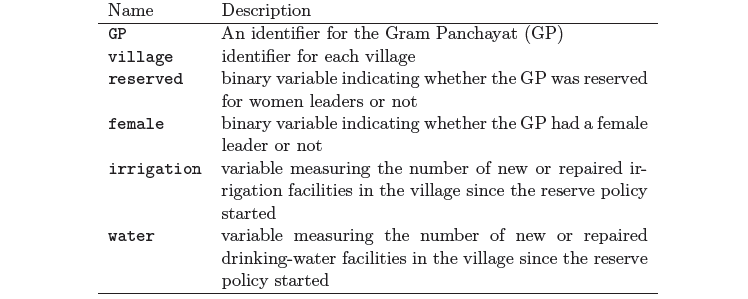
\includegraphics[width=1.1\textwidth]{women_desc.png}
\end{figure}		

\newpage
\begin{enumerate}
	\item [(a)] State a null and alternative (two-tailed) hypothesis. 
\\
\item HO: The reservation policy for women has no relation to more repaired drinking water facilities.
\item HA: The reservation policy for women has a relation to more repaired drinking water facilities.
	
	\vspace{.2cm}
	\item [(b)] Run a bivariate regression to test this hypothesis in \texttt{R} (include your code!).
	
I started of, after checking the dataframe in R, by boxplotting the water and reservation policy to get a vague understanding of any differences etc.
\begin{verbatim}
	ls(df)  #getting an overview  
	View(df) #getting an overview	
	boxplot(water ~ female, data = df, main = "res. vs. no-res.", ylim = c())
	#the outliers make the boxplot quite unreadable =  ylim will be set
\end{verbatim}

This is the boxplot:
\includegraphics[width=.6\textwidth]{ps02plot1.pdf}

The difference between reserved (1) and unreserved (0) is not strikingly if we look at the mean. Furthermore (for better visualisation) I excluded some outliers by setting the max. scale of Y to 60. Nevertheless, the correlation test had to be run to do the hypothesis test.


\newpage
\begin{verbatim}
correlation <- cor(df$water, df$reserved, method = "pearson") 
#correlation function
correlation

corrtest <- cor.test(df$water, df$reserved) #correlation test for more info
corrtest

summary(lm(df$water~df$reserved)) #getting the crucial data
	\end{verbatim}

By running the summary for lm we get these values.

\begin{verbatim}
Call:lm(formula = df$water ~ df$reserved)
Residuals:    
Min      1Q  
Median      3Q     
Max -23.991 -14.738  -7.865   2.262 316.009 
Coefficients:            
Estimate Std. Error t value Pr(>|t|)    
(Intercept)   14.738      2.286   6.446 4.22e-10 ***
df$reserved    9.252      3.948   2.344   0.0197 *  

---Signif. codes:  0 ‘***’ 0.001 ‘**’ 0.01 ‘*’ 0.05 ‘.’ 0.1 ‘ ’ 1
Residual standard error: 33.45 on 320 degrees of freedom
Multiple R-squared:  0.01688,	Adjusted R-squared:  0.0138 
F-statistic: 5.493 on 1 and 320 DF,  p-value: 0.0197
\end{verbatim}
Therefore, we would also reject the H0.

Following values indications were calculated  \textbf{Correlation: 0.1299079, and the p-value: 0.0197} as well as the confidence intervall with 95percent of: \textbf{lower:  0.02090616 higher: 0.23585751}. \\

As the p-value of 0.02 is lower than 0.05 we have evidence to reject the H0 and to accept HA.

	\vspace{.5cm}
	\item [(c)] Interpret the coefficient estimate for reservation policy. 
	
	The correlation of \textbf{0.1299079} is small but it shows a positive correlation between reservation for women and established water facilities. The y-intercept at 0 is 14.738 water installations. By increasing by 1 reservation, additional 9.252 water installations, on average, may be installed. Degrees of freedom indicate that there is more power and therefore the result can be significant (\href{https://sites.utexas.edu/sos/degreesfreedom/}{www.sites.utexas.edu})
	
	Concluding: We might have evidence that there is a relation between reservation policy for women and construction of drinking water facilities.
	

	
\end{enumerate}

\end{document}
